% Created 2020-02-27 Thu 14:37
% Intended LaTeX compiler: pdflatex
\documentclass[presentation]{beamer}
\usepackage[utf8]{inputenc}
\usepackage[T1]{fontenc}
\usepackage{graphicx}
\usepackage{grffile}
\usepackage{longtable}
\usepackage{wrapfig}
\usepackage{rotating}
\usepackage[normalem]{ulem}
\usepackage{amsmath}
\usepackage{textcomp}
\usepackage{amssymb}
\usepackage{capt-of}
\usepackage{hyperref}
\usetheme{metropolis}
\usecolortheme{}
\usefonttheme{}
\useinnertheme{}
\useoutertheme{}
\author{Petru Rebeja, Marius Apetrii}
\date{20 Februarie 2020}
\title{Tehnici Avansate de Programare}
\subtitle{Recapitulare și noțiuni de bază}
\institute[UAIC]{Facultatea de Matematică\\Universitatea Alexandru Ioan Cuza, Iași}
\hypersetup{
 pdfauthor={Petru Rebeja, Marius Apetrii},
 pdftitle={Tehnici Avansate de Programare},
 pdfkeywords={},
 pdfsubject={},
 pdfcreator={Emacs 26.3 (Org mode 9.3.6)},
 pdflang={Romanian}}
\begin{document}

\maketitle
\section{Introducere}
\label{sec:org39a9d24}
\begin{frame}[label={sec:orgf6925c4}]{Ce am discutat data trecută}
\pause
\begin{itemize}
\item Ciclul de dezvoltare al aplicațiilor
\item Dezvoltarea în iterații
\item Unelte de lucru
\item Fluxul de lucru Git
\item Bune practici
\end{itemize}
\end{frame}
\begin{frame}[label={sec:org55e29c5},fragile]{Ce vom discuta azi}
 \begin{itemize}
\item Tipuri de date în \texttt{.net}
\item Principiile programării orientată-obiect
\item Clase abstracte vs. interfețe.
\item Acuplare și Coeziune.
\end{itemize}
\end{frame}
\section{Tipuri de date în \texttt{.net}}
\label{sec:orgaed4876}
\begin{frame}[label={sec:orgbb5567a},fragile]{Tipuri \texttt{referință} și tipuri \texttt{valoare}}
 \begin{center}
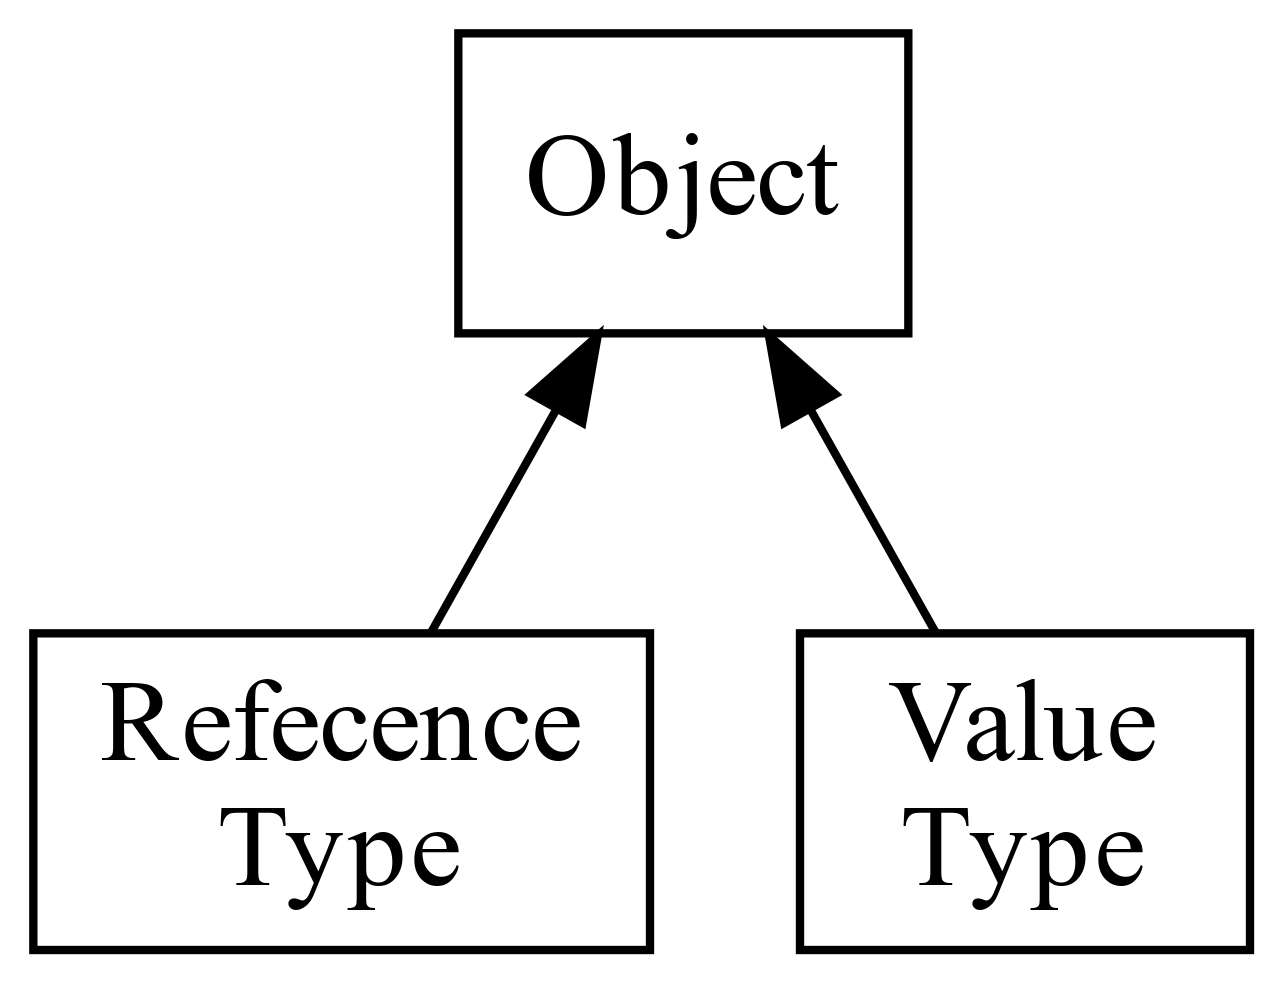
\includegraphics[width=0.6\textwidth]{./img/netcore-types.png}
\end{center}
\end{frame}
\begin{frame}[label={sec:orgc6c8715},fragile]{Tipuri \texttt{referință} și tipuri \texttt{valoare}}
 \begin{block}{Exemple}
\begin{center}
\begin{tabular}{ll}
Tip Referință & Tip Valoare\\
\hline
\texttt{string} & \texttt{int}\\
\texttt{System.Object} & \texttt{float}\\
\texttt{System.Action} & \texttt{bool}\\
\texttt{System.IO.MemoryStream} & Tipuri \texttt{struct}\\
\texttt{System.Collections.Generic.List<T>} & Tipuri \texttt{enum}\\
\end{tabular}
\end{center}
\end{block}
\end{frame}
\begin{frame}[label={sec:org4a38277},fragile]{Tipuri \texttt{valoare}}
 \begin{itemize}
\item O variabilă a unui tip valoare conține o instanță a tipului respectiv.
\item La crearea unei instanțe se alocă o singură zonă în memorie.
\item Dimensiunea zonei alocate este dată de tip.
\end{itemize}
\end{frame}
\begin{frame}[label={sec:orgc08bfea},fragile]{Tipuri \texttt{referință}}
 \begin{itemize}
\item O variabilă a unui tip referință conține adresa de memorie unde este alocată instanța propriu-zisă.
\item La crearea unei instanțe se alocă două zone de memorie:
\begin{itemize}
\item O zonă pentru adresă (stivă),
\item O zonă pentru instanță (memoria heap).
\end{itemize}
\item Dimensiunea zonei alocate pentru instanță poate să varieze (ex. \texttt{List<T>}).
\end{itemize}
\end{frame}
\begin{frame}[label={sec:org72fdd3b},fragile]{Cazul special: \texttt{string}}
 \begin{itemize}
\item Deși tipul \texttt{string} este un tip referință, acesta se comportă ca un tip valoare.
\item Această proprietate se numește \texttt{imuabilitate}
\end{itemize}
\end{frame}
\section{Principiile Programării Orientate-Obiect}
\label{sec:org6c50ecf}
\begin{frame}[label={sec:org30e7bd9}]{Recapitulare}
\begin{itemize}
\item \alert{Încapsularea} --- îmbinarea datelor și metodelor care le procesează.
\item \alert{Moștenire} --- proprietățile tipului părinte se păstrează și la copii.
\item \alert{Polimorfism} --- același comportament manifestat de mai multe tipuri.
\end{itemize}
\end{frame}
\begin{frame}[label={sec:orgc820c1a}]{Exemplificare}
\begin{block}{Context}
\vskip 0.1in
Pentru exemplificare vom modela o serie de operațiuni bancare.
\end{block}
\end{frame}
\begin{frame}[label={sec:orgda2c780}]{Exemplificare}
\begin{block}{Cerință I}
\vskip 0.1in
În calitate de posesor al unui cont bancar vreau să pot depune și extrage diverse sume de bani din cont.
\end{block}
\end{frame}
\begin{frame}[label={sec:org3d408fe}]{Încapsularea}
În situația de față, \alert{încapsularea} ne permite să îmbinăm retragerea de fonduri cu verificarea dacă sunt fonduri suficiente.
\end{frame}
\begin{frame}[label={sec:orgf303672}]{Exemplificare}
\begin{block}{Cerință II}
\vskip 0.1in
În calitate de posesor de conturi, pot avea conturi de diferite tipuri: economii și debit. Pentru retragerea de fonduri din fiecare cont se percep comisioane diferite în funcție de tipul acestuia:
\begin{itemize}
\item Pentru contul de debit: 0 \%
\item Pentru contul de economii: 0.5 \%
\end{itemize}
\end{block}
\end{frame}
\begin{frame}[label={sec:org03846c7}]{Exemplificare}
\begin{block}{Cerință III}
\vskip 0.1in
În calitate de posesor de conturi pot avea un cont de credit cu un comision de retragere de 0.7\%
\end{block}
\end{frame}
\begin{frame}[label={sec:org223cb78}]{Moștenirea}
În exemplul dat \alert{moștenirea} ne permite să declarăm o clasă de bază cu proprietățile comune și să implementăm particularitățile în clasele derivate.
\end{frame}
\begin{frame}[label={sec:org7f74662}]{Polimorfismul}
\alert{Polimorfismul} ne permite să aplicăm reguli de calcul diferite pentru aceeași metodă.
\end{frame}
\section{Clase abstracte vs. Interfețe}
\label{sec:orgfda11d5}
\begin{frame}[label={sec:org0628fac}]{Clasa abstractă}
\begin{itemize}
\item Oferă o implementare implicită pentru metode și proprietăți.
\item Nu se pot crea instanțe ale claselor abstracte.
\item Este mai puțin abstractă decât înterfața.
\item Poate impune anumite constrângeri (ex. constructorul).
\item Un tip de date poate deriva dintr-o singură clasă abstractă.
\end{itemize}
\end{frame}
\begin{frame}[label={sec:org6925415}]{Interfața}
\begin{itemize}
\item Nu oferă nicio implementare.
\item Cel mai mare grad de abstractizare.
\item Nu impune constrângeri decât asupra semnăturii metodelor.
\item Un tip de date poate implementa mai multe interfețe.
\end{itemize}
\end{frame}
\section{Modularizarea codului-sursă}
\label{sec:org83d0346}
\begin{frame}[label={sec:org976a385}]{Acuplare și Coeziune}
Două atribute foarte importante ale unui produs software de succes sunt:
\begin{itemize}
\item Grad mic de acuplare,
\item Grad mare de coeziune.
\end{itemize}
\end{frame}
\begin{frame}[label={sec:org8daeb39}]{Acuplarea}
\begin{quotation} %% Acuplarea
\alert{Acuplarea} este o măsură a gradului de interdependență dintre modulele unui produs software\footnote{\url{https://en.wikipedia.org/wiki/Coupling\_(computer\_programming)}}.
\end{quotation}
\end{frame}
\begin{frame}[label={sec:org934f8f6},fragile]{Acuplarea --- exemplu}
 Implementarea clasică a șablonului \texttt{Singleton} este un exemplu de grad înalt de acuplare: clasele care folosesc metodele definite de \texttt{Singleton} sunt dependente de acesta.
\end{frame}
\begin{frame}[label={sec:org2b86433}]{Coeziunea}
\begin{quotation} %% Coeziunea
\alert{Coeziunea} este măsura în care elementele unui modul aparțin unul de celălalt\footnote{\url{https://en.wikipedia.org/wiki/Cohesion\_(computer\_science)}}.
\end{quotation}
\end{frame}
\section{Încheiere}
\label{sec:orgda7319c}
\begin{frame}[label={sec:orgc949043},fragile]{Ce am discutat azi}
 \begin{itemize}
\item Tipuri de date în \texttt{.net}.
\item Principiile programării orientată-obiect.
\item Clase abstracte vs. interfețe.
\item Acuplare și Coeziune.
\end{itemize}
\end{frame}
\begin{frame}[label={sec:org517a0f1}]{Vă mulțumesc!}
\end{frame}
\end{document}